\section{Experiment and Analysis}
\label{sec:experiment}
The following experiment will measure several architectural-independent metrics of \SA solver and evaluate the architectural characteristics. Section~\ref{sec:setup} will introduce the experiment environment first. The experiment would be classified into three categories: Section~\ref{sec:computation} analyzes the computation resource related metrics including various instruction ratio, branch misprediction rate, floating point operation ratio, etc. Section~\ref{sec:memory} presents the result of memory footprint including the memory utilization, memory-related instruction ratio and cache miss rate. Section~\ref{sec:comparison} will make comparison of the two versions of \SA solvers with respect to the decrease of accuracy and the change of performance.
\subsection{Experiment Setup}
\label{sec:setup}
The experiment is carried out by a C-language \SA solver under 32-bit GNU/Linux 2.6.43. The CPU is Intel Core i7-2600@3.40GHz with 4 cores. L1 cache includes a 4 $\times$ 32 KB instruction cache and 4 $\times$ 32 KB data cache. L2 cache is 4 $\times$ 256 KB while the shared L3 cache is 8 MB. The input data sets were generated randomly and classified into three categories according to different sizes as in Table~\ref{tab:sizes}.

\begin{table}
  \centering
  \begin{tabular}{|l|l|l|}\hline
  \textbf{Data Set} & \textbf{Text file size} & \textbf{Number of equations}\\\hline
  Small & 19KB & 128 \\\hline
  Middle&127KB&512\\\hline
  Large&148KB&1024\\\hline
  \end{tabular}
  \caption{Size of different data sets}\label{tab:sizes}
\end{table}

\subsection{Computation Resource}
\label{sec:computation}
Computation Resource includes the ratio of different kind of instructions as well as other categories of CPU-related metrics such as memory/branch instruction ratios, branch misprediction rate under different prediction strategies etc. This part of metrics are measured by the binary instrument framework Pin-Tool and the performance evaluation tools VTune Amplifier provided by Intel. The following statistics are collected by running the solver using the different data sets except where noted.
\subsubsection{Instruction Ratio}
In this part I measure the ratio of memory and branch related instructions to reveal the effect of jump/branch instructions to the overall performance. The statistics is shown in the Figure~\ref{fig:ratio}.
\begin{figure}
\centering
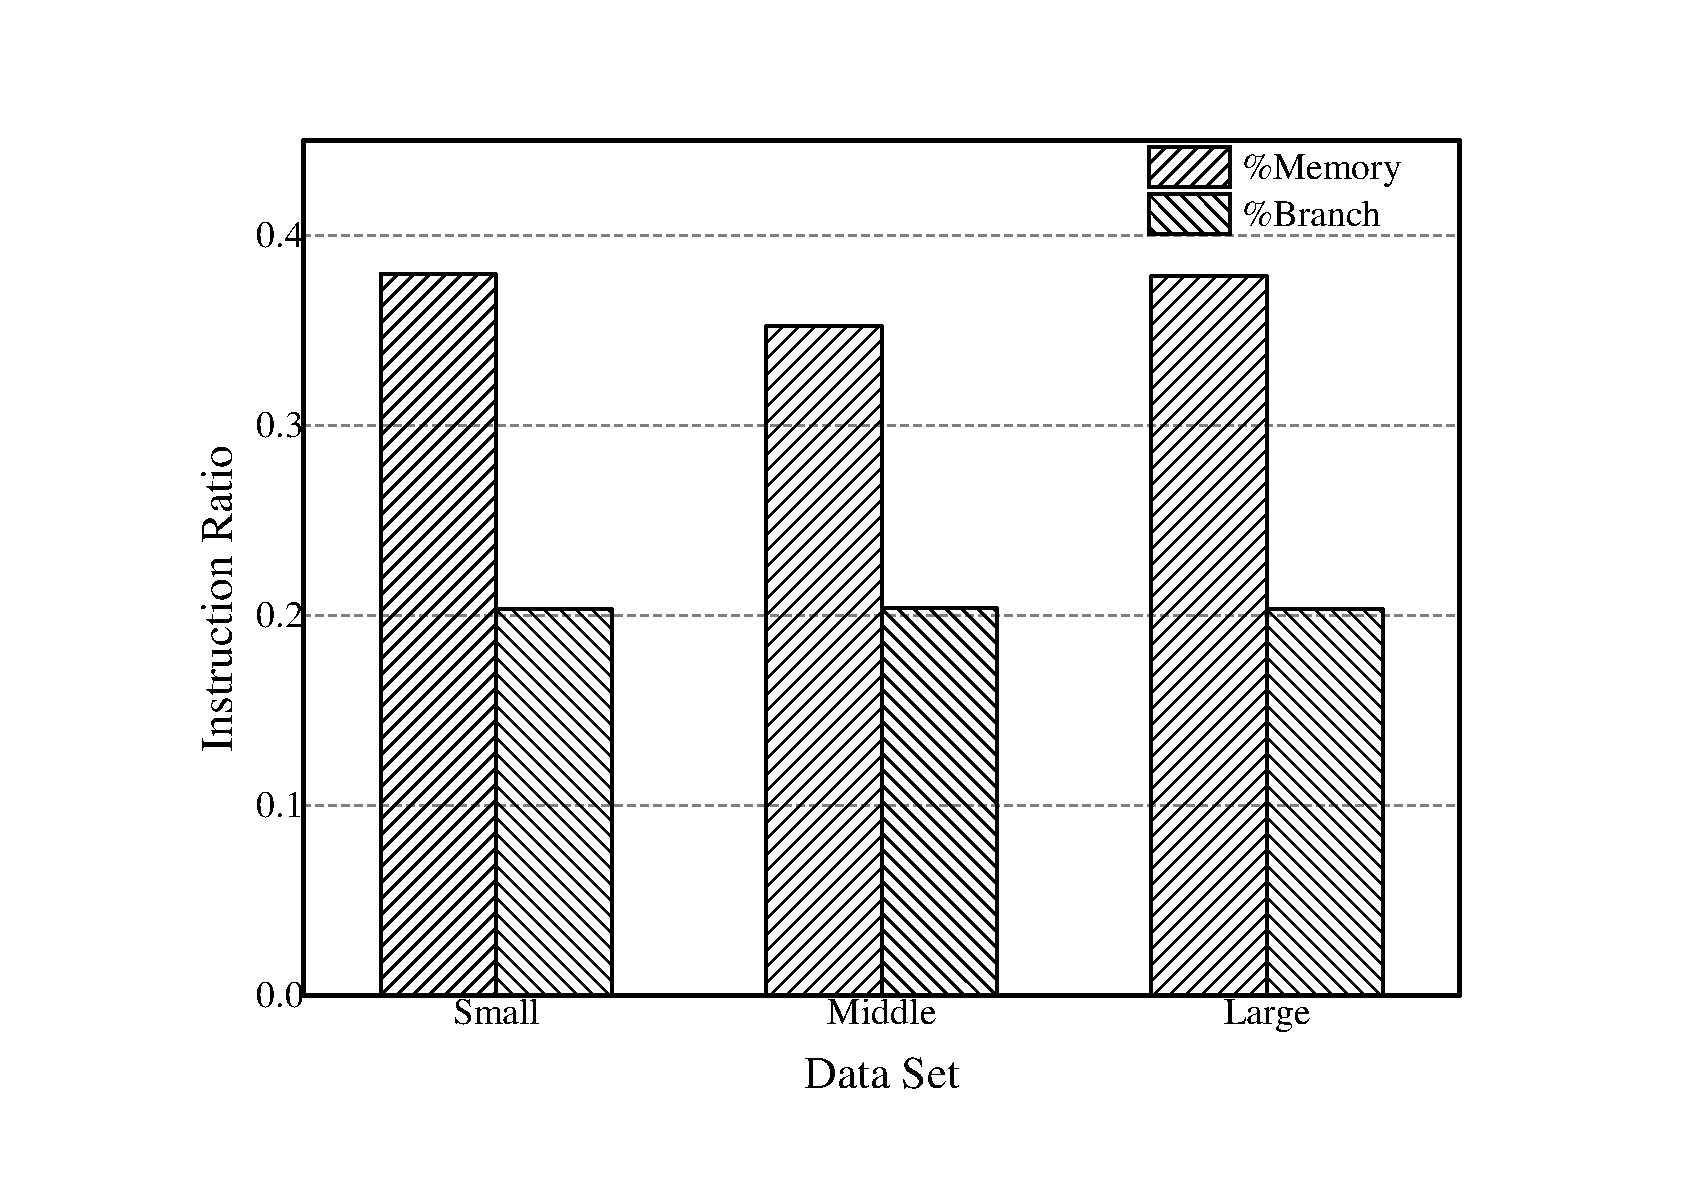
\includegraphics[width=0.50\textwidth]{graph/ins_ratio.pdf}
\caption{Instruction Ratio.}
\label{fig:ratio}
\end{figure}
\subsubsection{Branch Misprediction Ratio }
\subsection{Memory Footprint}
\label{sec:memory}
\subsection{Comparison of Two Versions}
\label{sec:comparison} 